
\documentclass[addpoints,12pt]{exam}

\usepackage{amsmath}
\usepackage{amsthm}
\usepackage{graphicx}
\usepackage{enumitem}
\usepackage{amssymb}
\usepackage{tikz}
\usepackage{multicol}
\usepackage{comment}
\usepackage{geometry}

\noprintanswers %Remove to hide answers
\pagestyle{headandfoot} %Adds Headers and Footers
\runningheadrule
\firstpageheader{Math 125}{Exam 1 }{\today}
\runningheader{Math 125}
{Exam 1, Page \thepage\ of \numpages}
{\today}
\firstpagefooter{}{\thepage}{}
\runningfooter{}{\thepage}{}

\newcommand{\tft}{
\begin{oneparcheckboxes}
\CorrectChoice True
\choice False
	\end{oneparcheckboxes}
}
\newcommand{\tff}{
\begin{oneparcheckboxes}
\choice True
\CorrectChoice False
	\end{oneparcheckboxes}
}

\checkboxchar{$\Box$}
\checkedchar{$\blacksquare$}


\begin{document}

%The box at the top, and the name
\begin{center}
\fbox{\fbox{\parbox{5.5in}{\centering
Answer the questions in the spaces provided on the
question sheets. If you run out of room for an answer,
continue on the back of the page.}}}
\end{center}
\vspace{0.1in}
\makebox[\textwidth]{Name:\enspace\hrulefill}
\vspace{0.2in}

%Question Formatting
%\qformat{\textbf{Question \thequestion}\quad (\thepoints)\hfill}
%Point Table
\newtheorem{theorem}{Theorem}

%\begin{center}
%\gradetable[h][questions]
%\end{center}

%Beginning Questions
\begin{questions}
	\question Answer each of the following. \begin{enumerate}[label=\alph*)]
	    \item Give an example of a finite set $A$ in set builder notation. \vfill
			\item Write this same set $A$ in roster method. \vfill
			\item Give the cardinality $n(A)$ of your finite set $A$. \vfill
			\item Give an example of a proper subset of your set $A$ if it exists. If there does not exist a proper subset, state why. Be sure to use proper notation when naming your subset, either using roster or set builder notation. \vfill
			\item Is the set $\emptyset$ a subset of your set $A$?
	\end{enumerate} \vfill



	\question Consider the following two sets 
	\[
	A=\{1,2,3,4,5,6\} \hspace{30pt} B = \{4,5,6,7,8\}
	\]
	Answer the following True or False questions. 
	\begin{enumerate}[label = \alph*)]
		\item \tff $A\subseteq B$
		\item \tft $A\cap B = \{4,6\}$
		\item \tff $A\cup B = \{1,2,3,4,5,6,7,8\}$
		\item \tft $\{1,2,3,4,5,6\} \subset A$ 
		\item \tft $A\cap B \subseteq A\cup B$
		\item \tff $2\in A$ and $6\in B$ 
	\end{enumerate}

	\newpage

\question
Shade in the indicated subset in each Venn Diagram. 

\begin{multicols}{2}

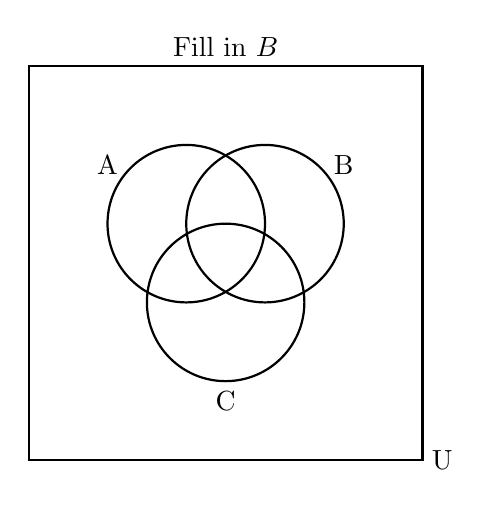
\begin{tikzpicture}
	\draw[black,thick] (0,0) rectangle (5,5) ;
\draw[black,thick] (2,3) circle (1);
\draw[black, thick] (3,3)circle (1);
\draw[black,thick] (2.5,2) circle (1);
\node (A) at (1,3.75){A};
\node (B) at (4,3.75){B};
\node (C) at (2.5,0.75) {C};
\node (U) at (5.25,0) {U};
\node (D) at (2.5,5.25) {Fill in $B$};
\end{tikzpicture}

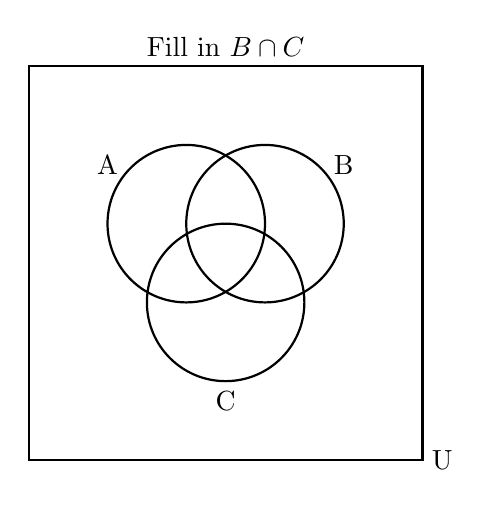
\begin{tikzpicture}
	\draw[black,thick] (0,0) rectangle (5,5) ;
\draw[black,thick] (2,3) circle (1);
\draw[black, thick] (3,3)circle (1);
\draw[black,thick] (2.5,2) circle (1);
\node (A) at (1,3.75){A};
\node (B) at (4,3.75){B};
\node (C) at (2.5,0.75) {C};
\node (U) at (5.25,0) {U};
\node (D) at (2.5,5.25) {Fill in $B\cap C$};

\end{tikzpicture}

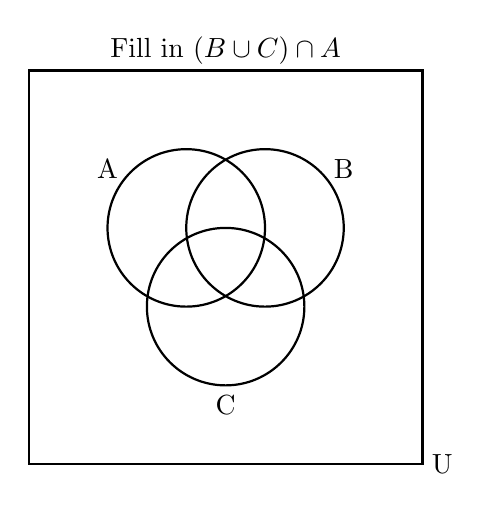
\begin{tikzpicture}
	\draw[black,thick] (0,0) rectangle (5,5) ;
\draw[black,thick] (2,3) circle (1);
\draw[black, thick] (3,3)circle (1);
\draw[black,thick] (2.5,2) circle (1);
\node (A) at (1,3.75){A};
\node (B) at (4,3.75){B};
\node (C) at (2.5,0.75) {C};
\node (U) at (5.25,0) {U};

\node (D) at (2.5,5.25) {Fill in $(B\cup C)\cap A$};

\end{tikzpicture}

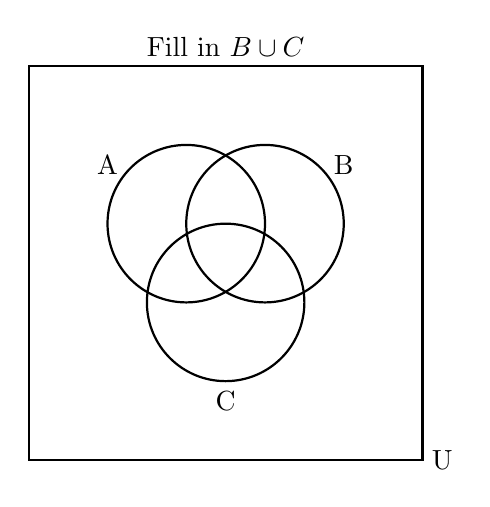
\begin{tikzpicture}
	\draw[black,thick] (0,0) rectangle (5,5) ;
\draw[black,thick] (2,3) circle (1);
\draw[black, thick] (3,3)circle (1);
\draw[black,thick] (2.5,2) circle (1);
\node (A) at (1,3.75){A};
\node (B) at (4,3.75){B};
\node (C) at (2.5,0.75) {C};
\node (U) at (5.25,0) {U};

\node (D) at (2.5,5.25) {Fill in $B\cup C$};

\end{tikzpicture}

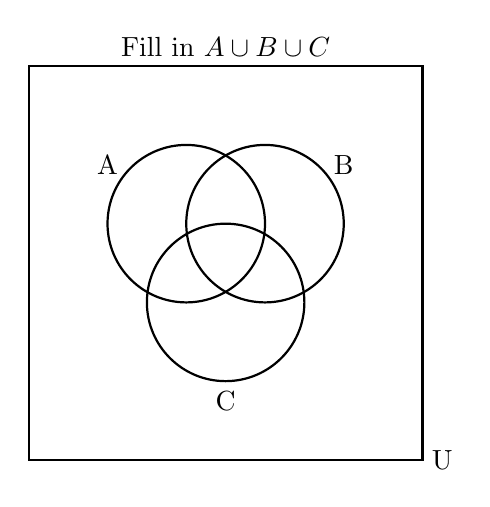
\begin{tikzpicture}
	\draw[black,thick] (0,0) rectangle (5,5) ;
\draw[black,thick] (2,3) circle (1);
\draw[black, thick] (3,3)circle (1);
\draw[black,thick] (2.5,2) circle (1);
\node (A) at (1,3.75){A};
\node (B) at (4,3.75){B};
\node (C) at (2.5,0.75) {C};
\node (U) at (5.25,0) {U};

\node (D) at (2.5,5.25) {Fill in $A\cup B\cup C$};

\end{tikzpicture}

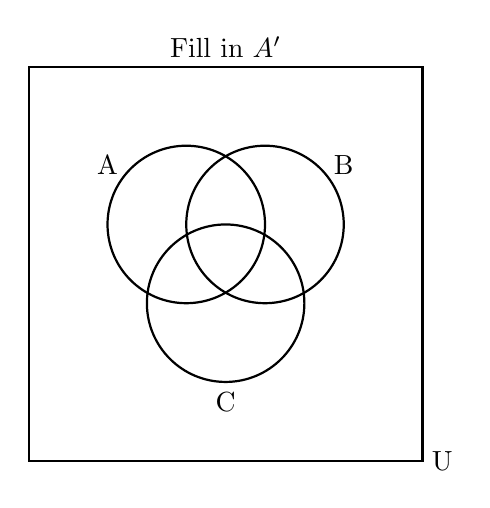
\begin{tikzpicture}
	\draw[black,thick] (0,0) rectangle (5,5) ;
\draw[black,thick] (2,3) circle (1);
\draw[black, thick] (3,3)circle (1);
\draw[black,thick] (2.5,2) circle (1);
\node (A) at (1,3.75){A};
\node (B) at (4,3.75){B};
\node (C) at (2.5,0.75) {C};
\node (U) at (5.25,0) {U};

\node (D) at (2.5,5.25) {Fill in $A'$};

\end{tikzpicture}

\end{multicols}

\newpage

\question Consider a poll where 44 people are asked if they eat Sauerkraut, Kimchi, and Miso. Let $A$ be the set of people that like Sauerkraut, $B$ be the set of people that like Kimchi, and $C$ be the set of people that like Miso. Consider the following pieces of information
\begin{itemize}
	\item We know 16 people like Sauerkraut. 
	\item We know 13 people like Kimchi. 
	\item We know 22 people like Miso.
	\item We know 6 people like Saurkraut and Kimchi
	\item We know 11 people like Sauerkraut and Miso. 
	\item We know 9 people like Kimchi and Miso. 
	\item We know 3 people like all 3. 
\end{itemize}

Fill in each region of the Venn Diagram with the number of people in each region. 

\begin{center}
$A\sim \text{Sauerkraut} \hspace{20pt} B \sim \text{Kimchi}\hspace{20pt} C \sim \text{Miso}$ 

\vspace{10pt}

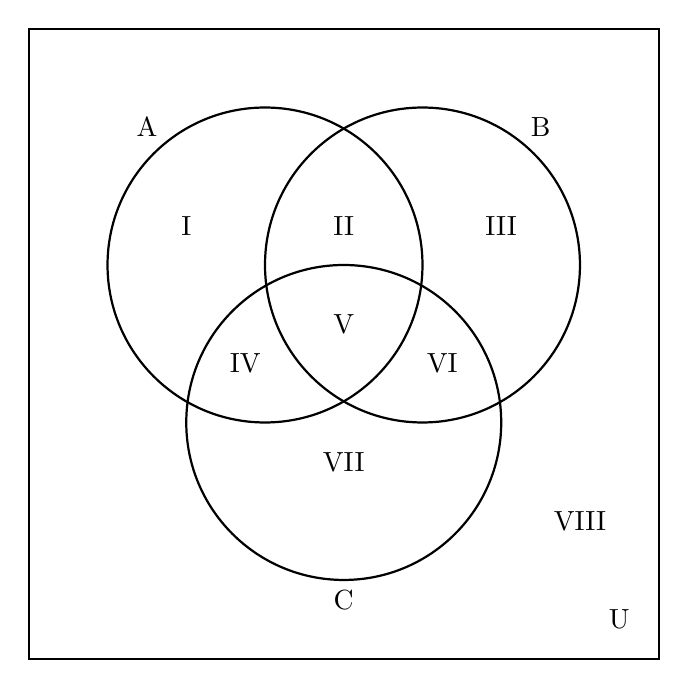
\begin{tikzpicture}
\draw[black,thick] (0,0) rectangle (8,8) ;
\draw[black,thick] (3,5) circle (2);
\draw[black, thick] (5,5) circle (2);
\draw[black,thick] (4,3) circle (2);
\node (A) at (1.5,6.75){A};
\node (B) at (6.5,6.75){B};
\node (C) at (4,0.75) {C};
\node (U) at (7.5,0.5) {U};
\node (3) at (2,5.5) {I};
\node (3) at (6,5.5) {III};
\node (3) at (4,5.5) {II};
\node (3) at (2.75,3.75) {IV};
\node (3) at (5.25,3.75) {VI};
\node (3) at (4,2.5) {VII};
\node (3) at (4,4.25) {V};
\node (3) at (7,1.75) {VIII};
\end{tikzpicture}
\end{center}

\newpage

\question Use the accompanying Venn diagram, which gives the cardinality of each region, to answer the questions below. Feel free to leave answers unsimplified! 

\begin{enumerate}[label = \alph*)]
    \item How many elements below to set $B$? 
		\item How many elements belong to $A$ but not to $B$, that is, what is $n(A\cap B ')$?
		\item How many elements belong to set $A$ or set $B$,  that is, what is $n(A\cup B)$? 
		\item How many elements below to $B$ and $C$, that is, what is $n(B\cap C)$ ?
		\item How many elements belong in at least $1$ of the sets $A$, $B$ and $C$? that is, what is $n(A\cup B\cup C$)?

			Hint: $n(U) = 37$
\end{enumerate}

\begin{center}
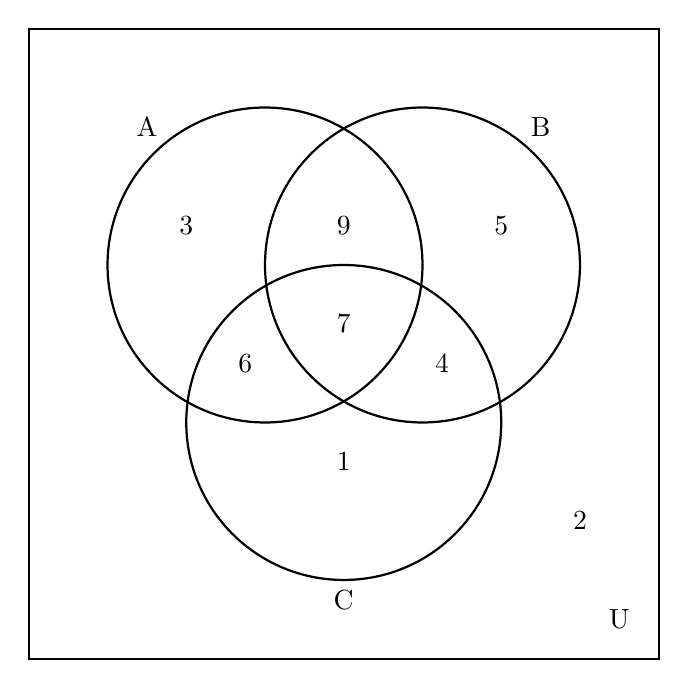
\begin{tikzpicture}
\draw[black,thick] (0,0) rectangle (8,8) ;
\draw[black,thick] (3,5) circle (2);
\draw[black, thick] (5,5) circle (2);
\draw[black,thick] (4,3) circle (2);
\node (A) at (1.5,6.75){A};
\node (B) at (6.5,6.75){B};
\node (C) at (4,0.75) {C};
\node (U) at (7.5,0.5) {U};
\node (3) at (2,5.5) {3};
\node (3) at (6,5.5) {5};
\node (3) at (4,5.5) {9};
\node (3) at (2.75,3.75) {6};
\node (3) at (5.25,3.75) {4};
\node (3) at (4,2.5) {1};
\node (3) at (4,4.25) {7};
\node (3) at (7,1.75) {2};
\end{tikzpicture}
\end{center}


\newpage
\question You take a poll of $50 $ college students where classes at their college are held either Monday, Wednesday and Friday(MWF), or classes are help Tuesday and Thursday (TR). Assume every student is taking at least one class (they are students after all). If $25$ students report having classes MWF and $30$ students report having classes on TR, how many people have class every day of the week? Hint: Use the inclusion-exclusion principle. 


\begin{theorem}[Inclusion-Exclusion Principle]
		\[
		n(A\cup B) = n(A)+n(B)-n(A\cap B)
		\]
\end{theorem}\vfill 

\question  What is your current favorite song? \vfill


\end{questions}
\end{document}
